% ============================================================
%  B2Z UC1 4页会议论文 — 中文同步版主文件
%  编译：cd paper/zh && latexmk -xelatex -interaction=nonstopmode -halt-on-error main_zh.tex
%  产物：paper/build/zh/main_zh.pdf
%  共享资源：../figures/（矢量图）、../refs.bib（唯一文献库）
% ============================================================
\documentclass[conference]{IEEEtran}

\usepackage[super,nomove]{cite}
\let\ITCAcitefont\OverciteFont
\renewcommand{\OverciteFont}[1]{\ITCAcitefont[#1]}
\usepackage{amsmath,amssymb,amsfonts}
\usepackage{graphicx}
\usepackage{booktabs}
\usepackage{multirow}
\usepackage{siunitx}
\usepackage{textcomp}
\usepackage{xcolor}
\usepackage{url}
\urlstyle{same}
\usepackage[hidelinks]{hyperref}

% 中文排版支持（保留 IEEEtran 双栏版面与数字/公式风格，与英文 4 页主版 1:1 对齐）
\usepackage[UTF8,scheme=plain,heading=false]{ctex}
\setCJKmainfont{Noto Serif CJK SC}[BoldFont=Noto Serif CJK SC Bold,ItalicFont=AR PL UKai CN]
\setCJKsansfont{Noto Sans CJK SC}
\setCJKmonofont{Noto Sans Mono CJK SC}
\XeTeXlinebreaklocale "zh"
\XeTeXlinebreakskip = 0pt plus 1pt

\renewcommand{\figurename}{图}
\renewcommand{\tablename}{表}
\renewcommand{\thetable}{\arabic{table}}
\renewcommand{\refname}{参考文献}
\renewcommand{\abstractname}{摘要}
\renewcommand{\IEEEkeywordsname}{关键词}

\graphicspath{{../figures/}}

\sisetup{
  detect-all,
  group-separator = {,},
  group-minimum-digits = 4,
  range-phrase = {--},
  range-units = single
}

% ---- 与英文版 main.tex 完全一致的术语宏 ----
\newcommand{\proto}{UC1}
\newcommand{\fragproto}{C3}
\newcommand{\modejc}{JC}
\newcommand{\modesc}{SC}
\newcommand{\modelc}{LC}
\newcommand{\ble}{BLE}
\newcommand{\stdfour}{IEEE~802.15.4}

\begin{document}

\title{低功耗蓝牙扩展广播中双协议共包控制的成本与联合解析权衡}

\author{\IEEEauthorblockN{吉志学\textsuperscript{*}}
\IEEEauthorblockA{\textit{计算机科学与工程学院} \\
\textit{电子科技大学}\\
中国成都 611730 \\
202421080910@std.uestc.edu.cn}
}

\maketitle

\begin{abstract}
从单一发送机同时控制共处同一频段的低功耗蓝牙（Bluetooth Low Energy）与 IEEE 802.15.4 接收机通常需要顺序发送多组突发及多帧传统分片，但其封装代价与双侧接收权衡尚缺乏定量刻画。本文提出一种共包双协议控制封装与解析式波形成本模型，基于 BlueBee 物理层仿真在单个低功耗蓝牙扩展广播次信道协议数据单元（protocol data unit）中嵌入可独立校验的命令及共享时隙时间元数据，并构造槽隔离传统分片基线作为对照。在双链软件定义无线电（software-defined radio）原型上的有线测试验证了三组记录布局（26/26、52/26 与 28/32 字节）的完整恢复、确定性包内时间偏移以及单侧断馈恢复能力。在 36 轮确认性无线实验（3,600 项计划任务）中，本文确立了三项结论：（1）在相等的单次尝试提交波形时长下，共包相对同频分别发送将每次尝试突发数由 3 个减至 2 个，而计划尝试内联合解析率未呈一致增益；（2）对于短记录，传统广播在单次尝试时单位波形成本最低，但在 6 ms 预算上限下传统广播发送 4 次而共包发送 3 次，成本排序发生翻转，共包单位成本降低 14.8\%；（3）对于 52 字节低功耗蓝牙记录，共包方案免除五分片重组，在 6 ms 上限下于信道 3 取得 291/300 联合解析，高于传统广播在信道 39 上的 93/300。
\end{abstract}

\begin{IEEEkeywords}
低功耗蓝牙，扩展广播，IEEE 802.15.4，跨技术通信，分片重组，软件定义无线电
\end{IEEEkeywords}

\section{引言与相关工作}\label{sec:intro}

室内传感与智能家居网络常在 \SI{2.4}{GHz} 频段并存部署低功耗蓝牙（\ble{}）~\cite{bluetooth_core51} 与 \stdfour{}~\cite{ieee802154_2020} 节点。在没有多电台网关的情况下，单一发送机向两类协议设备下发控制命令通常只能按协议顺序分别发送突发~\cite{brunner2021leveraging}，而超出 \SI{31}{B} 传统 \ble{} 广播净荷上限的命令还必须跨多帧分片。无连接 \ble{}~5.1 扩展广播将至多 \SI{255}{B} 卸载至次信道 \texttt{AUX\_ADV\_IND} 协议数据单元（PDU）~\cite{bluetooth_core51}，从而使单个次信道突发能够同时承载独立命令与共享时间元数据。

既有跨技术通信（CTC）研究已覆盖物理层帧仿真（BlueBee~\cite{jiang2017bluebee} 将 \stdfour{} 码片映射至 \SI{1}{Mbps} \ble{} 高斯频移键控（GFSK）比特，带来 $4\times$ 字节膨胀）、包级异构广播调度（Brunner 等人~\cite{brunner2021leveraging}）、宽带 IEEE~802.11ax 正交频分多址（OFDMA）并发传输（WiCast~\cite{xia2025wicast}），以及基于外部参考的物联网（IoT）设备双向时钟同步（X-Sync~\cite{hofmann2021xsync}、TimeBee~\cite{gao2023timebee}）。然而，针对不具备宽带 OFDMA 能力的单个 \SI{2}{MHz} 带宽 \ble{}~5 广播射频，既有工作尚未定量刻画：当单次任务要求\emph{双侧接收链均校验通过}各自独立命令时，共包封装开销、等预算重发行为以及传统广播分片暴露风险如何制约整体权衡。在不把双协议广播宣称为首次提出、不提出跨设备时钟同步算法、也不将本地预测误差与 X-Sync~\cite{hofmann2021xsync} 排名的前提下，本文研究固定次信道单个 \texttt{AUX\_ADV\_IND} 共包何时能够在提交波形成本与计划尝试内联合解析率上取得收益。

为在匹配的逻辑任务语义下回答该问题，本文设计了统一紧凑双协议封装（\proto{}）及槽隔离传统分片基线（\fragproto{}），并在单台软件定义无线电（SDR）发送机与两套独立 SDR 接收链上实现评估。本文形成三项有界贡献：（1）形式化给出 \proto{}/\fragproto{} 帧布局、解析式提交波形成本模型以及确定性包内标记偏移，并通过有线馈线实采完成验证；（2）通过 36 轮交替区组无线实验（\num{3600} 项计划任务），在相等单次尝试波形时长下隔离共包带来的突发次数缩减（\modejc{} 对 \modesc{}，同用 \ble{} ch3 / \stdfour{} ch12），并定量揭示相对 ch39 \modelc{} 由载荷与预算策略驱动的单位成本排序翻转及分片损益；（3）评估固定次信道时间可用性与单侧断馈恢复行为（第~\ref{sec:design}--\ref{sec:eval} 节、图~\ref{fig:layout}--\ref{fig:p4_tradeoff}、表~\ref{tab:budget}--\ref{tab:p4_main}）。

% 按英文 4 页会议主版结构，相关工作已并入第一节（02-related-work.tex 保留备查）：
% \section{相关工作与研究边界}\label{sec:related}

跨技术通信按作用层次可分为物理层仿真与包级/多载波并发广播两类。在物理层方向，BlueBee~\cite{jiang2017bluebee} 利用 \SI{1}{Mbps} \ble{} 高斯频移键控（GFSK）波形构造 \stdfour{} 合法码片序列，每字节 \stdfour{} 帧需占用 $4$ 字节 \ble{} 载荷，并在商用芯片上实现了双标准兼容帧解析与智能灯具控制；其期刊扩展版进一步面向商用物联网设备提升了跨技术通信比特率~\cite{jiang2019boosting}。在包级与多协议广播方向，Brunner 等人~\cite{brunner2021leveraging} 基于包级能量突发（X-Burst）与原生协议栈共存调度，实现了由智能手机无网关控制 \ble{} 门锁与 ZigBee 灯具的异构智能家居原型；WiCast~\cite{xia2025wicast} 则在 IEEE~802.11ax（Wi-Fi~6）正交频分多址（OFDMA）单个资源单元上合成复合信号，并行服务 \ble{}、ZigBee 与 LoRa 接收端。与上述工作不同，本文聚焦于单个 \SI{2}{MHz} 带宽 \ble{}~5 扩展广播发送机约束，既不依赖宽带 Wi-Fi OFDMA 发射端，也不把双协议广播本身视作首次提出，而是定量评估在单个 \texttt{AUX\_ADV\_IND} 中并置双侧结构化控制记录与时间元数据时的布局开销、波形成本与联合解析权衡。

在跨技术时间分发方向，专用同步协议致力于实现异构节点间亚毫秒乃至微秒级绝对时钟对齐。X-Sync~\cite{hofmann2021xsync} 在商用 \ble{} 与 \stdfour{} 节点间采用变长能量突发与重复接收信号强度（RSS）二分搜索，借助外部参考测得微秒级跨设备时钟偏差；Crocs~\cite{yu2018crocs} 与 TimeBee~\cite{gao2023timebee} 面向 Wi-Fi 与 ZigBee 共存网络设计了跨技术时间同步框架。本文并不提出新的跨设备时钟同步算法，也不将本系统的测量值与 X-Sync 等同步精度指标直接排名：本文将共享时隙参考元数据附属嵌入单向共包控制流，仅在固定次信道下评估单侧接收机本侧 IQ 采样域的留出预测残差、未知外部参考界下的保守拒绝以及单侧失更后的状态恢复行为。

\ble{}~5.1 核心规范定义的扩展广播机制~\cite{bluetooth_core51} 将主信道指针与次信道长载荷解耦，突破了传统广播 \SI{31}{B} 荷载限制。为保证实验归因清晰并遵守测量边界，本文在设计阶段明确以下范围与非目标：确认性实验在固定次信道上开展（不将动态 \texttt{AuxPtr} 切频跟随瞬态与在线时间机制混同），其中 \modejc{} 与 \modesc{} 的 \ble{} 侧均使用 ch3（\SI{2410}{MHz}）、\stdfour{} 侧均使用 ch12（\SI{2410}{MHz}），构成同频可协议归因对照；而 \modelc{} 的 \ble{} 侧位于传统广播信道 ch39（\SI{2480}{MHz}），因此 \modejc{}--\modelc{} 的联合解析率差异仅对应所测封装与信道组合。此外，所有成本均以提交设计波形代理时长（\si{\micro\second}）核算，不宣称功率计实测射频空口时长或能耗；全部结果基于单 SDR 发送机与两套独立 HackRF 接收链，不宣称商用协议栈完整兼容或物理执行器同步动作。

\section{共包协议设计与对照封装}\label{sec:design}

\begin{figure}[t]
  \centering
  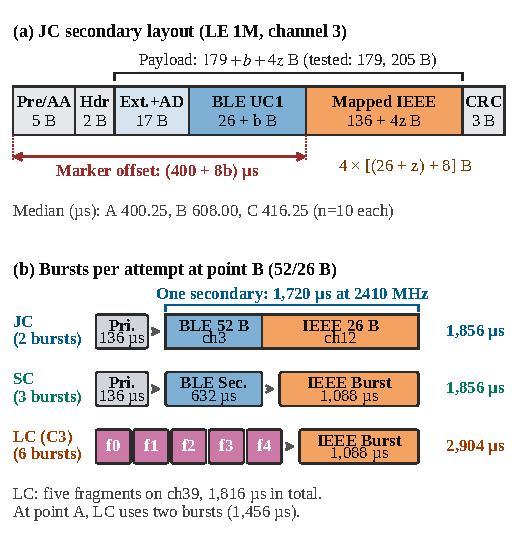
\includegraphics[width=\columnwidth]{fig-uc1-layout-bursts.pdf}
  \caption{统一紧凑格式（\proto{}）共包次信道数据单元布局与单次尝试突发对比：(a) \texttt{AUX\_ADV\_IND} 字节预算与确定性偏移 $\num{400}+8b\,\si{\micro\second}$；(b) B 点（$52/26$\,B）下 \modejc{}、\modesc{} 与需五片 \fragproto{} 分片的 \modelc{} 突发结构。}
  \label{fig:layout}
\end{figure}

\subsection{单发送机封装模式与字节/波形预算}\label{sec:design_modes}

发送机按 \SI{500}{ms} 时隙（$T_{\text{slot}}{=}\SI{500}{ms}$）向 \ble{} 接收链与 \stdfour{} 接收链调度发送尝试；在 P4 中，相邻逻辑任务的起始槽相隔 $6$ 个时隙（\SI{3}{s}）。每项逻辑任务由 $(\texttt{run\_id}, \texttt{command\_id})$ 唯一标识，在单向无确认信道下按固定计划尝试次数 $K$ 或共同单任务波形预算上限 $Q$（\si{\micro\second}）执行开环发送，每次物理尝试占据一个递增槽号 $\texttt{slot\_index}$。如图~\ref{fig:layout} 所示，本文在同一任务语义下实现三种封装模式：共包扩展广播（\modejc{}）每次尝试发射 $2$ 个突发，包括 $1$ 个主信道 \texttt{ADV\_EXT\_IND}（\SI{136}{\micro\second}）与 $1$ 个位于 \ble{} ch3（\SI{2410}{MHz}，与 \stdfour{} ch12 中心频点重合）的次信道 \texttt{AUX\_ADV\_IND}，在单帧中顺次容纳 \ble{} 记录与 BlueBee 映射后的 \stdfour{} 记录；同频分别扩展广播（\modesc{}）每次尝试发射 $3$ 个突发，即主信道指针、仅含 \ble{} 记录的 ch3 次信道帧以及独立的 ch12 BlueBee 映射 \stdfour{} 突发；传统广播/分片基线（\modelc{}）每次尝试发射 $F+1$ 个突发，在传统广播信道 ch39（\SI{2480}{MHz}）发送 $F$ 帧 \ble{} 广播后再于 ch12 发送 $1$ 个独立 \stdfour{} 突发。

在应用记录层，\ble{} 与 \stdfour{} 各自独立封装并校验一条长度为 $(26+n)$\,B 的小端 \proto{} 记录（\ble{} 侧 $n{=}b$，\stdfour{} 侧 $n{=}z$）。每条记录由 \SI{24}{B} 固定头（含 \texttt{magic=0xC1}、显式版本类型字节 \texttt{0x10} 纯时间更新或 \texttt{0x11} 控制命令、\texttt{run\_id}、\texttt{slot\_index}、\texttt{period\_ms}、\texttt{command\_id}、\texttt{target\_id}、\texttt{opcode}、\texttt{arg}、\texttt{valid\_offset\_ms}、\texttt{execute\_offset\_ms} 与 \texttt{extra\_len}）、$n$\,B 本侧扩展净荷以及 \SI{2}{B} \texttt{CRC-16/CCITT-FALSE} 校验构成。在 \modejc{} 冻结布局中，扩展广播头、Flags AD 与 Manufacturer AD 头共占 \SI{17}{B}，BlueBee 映射区占 $4(26+z+8)=136+4z$\,B（内含 \SI{8}{B} \stdfour{} PHY/MAC 封装），故次信道 PDU 载荷长度为
\begin{equation}\label{eq:sec_payload}
  L_{\text{sec}}(b,z) = 17 + (26 + b) + (136 + 4z) = 179 + b + 4z~\text{B}.
\end{equation}
受 \SI{255}{B} 次信道载荷协议上限约束，式~\eqref{eq:sec_payload} 的字节算术边界为 $b+4z\le 76$；本文阶段一冻结工作域限定为 $0\le b\le 26$、$0\le z\le 6$ 且满足共同约束 $b+4z\le 26$（两项边际最大值 $b{=}26$ 与 $z{=}6$ 不可组合）。实验选取三组代表配置（按 \ble{}/\stdfour{} 顺序）：短负载 A 点（扩展 $0/0$\,B，完整记录 $26/26$\,B，次信道载荷 \SI{179}{B}）、长 \ble{} 负载 B 点（扩展 $26/0$\,B，完整记录 $52/26$\,B，载荷 \SI{205}{B}）及双侧非对称负载 C 点（扩展 $2/6$\,B，完整记录 $28/32$\,B，载荷 \SI{205}{B}）；另设 B1 点（扩展 $1/0$\,B，完整记录 $27/26$\,B）核验传统广播 \SI{27}{B} 直接承载边界。

在 LE~1M 速率下，三种模式单次完整逻辑尝试的设计有效波形代理预算（\si{\micro\second}，不含包间静默与调谐保护间隔）如表~\ref{tab:budget} 所示，由下式精确给出：
\begin{align}
  C_{\modejc}(b,z) &= C_{\modesc}(b,z) = 1648 + 8b + 32z,\label{eq:cost_jc_sc}\\
  C_{\modelc}(b,z) &=
  \begin{cases}
    8(182 + b + 4z), & b \le 1,\\
    8(35F + 162 + b + 4z), & b \ge 2.
  \end{cases}\label{eq:cost_lc}
\end{align}
其中 \modelc{} 在 $b\le 1$ 时以单个 Manufacturer AD 直接承载完整 \ble{} 记录（$F{=}1$）；当 $b\ge 2$ 时进入 \fragproto{} 分片，每片含 \SI{20}{B} 传统广播空口封装与 \SI{15}{B} 分片头，最多承载 \SI{12}{B} 记录字节，分片数 $F=\lceil(26+b)/12\rceil$（B 点 $52$\,B 对应 $F{=}5$）。由式~\eqref{eq:cost_jc_sc} 可见，\modejc{} 与 \modesc{} 在任意 $(b,z)$ 下单次提交波形代理预算完全相等，而 \modejc{} 将每次尝试的突发数由 $3$ 次降至 $2$ 次。在同预算上限 $Q$ 策略下，各模式分配计划尝试次数 $K_m=\lfloor Q/C_m\rfloor$，并将剩余未用预算 $Q-K_m C_m$ 显式记录而不以无意义填充补齐。

% ============================================================
%  表 1（中文同步版）：与 ../tables/tab-budget.tex 数值 100% 同步
%  数据源：python/experiments/p5_freeze_20261124/p5_p2_h2_h3.csv
% ============================================================
\begin{table}[t]
\centering
\caption{代表性负载点的字节布局、单尝试提交波形代理预算与有线馈线核验。}
\label{tab:budget}
\setlength{\tabcolsep}{2.0pt}
\scriptsize
\begin{tabular}{@{}lccccccc@{}}
\toprule
\textbf{测点} & \textbf{记录} & \textbf{映射} & \textbf{\modejc{}载荷} & \multicolumn{3}{c}{\textbf{突发数 / 代理 (\si{\micro\second})}} & \textbf{偏移} \\
\cmidrule(lr){5-7}
$(b,z)$ & B/Z & (B) & (B) & \modejc{} & \modesc{} & \modelc{} ($F$) & (\si{\micro\second}) \\
\midrule
A $(0,0)$   & 26/26 & 136 & 179 & 2/\num{1648} & 3/\num{1648} & 2/\num{1456} (1) & 400.25 \\
B1 $(1,0)$  & 27/26 & 136 & 180$^{\mathrm{a}}$ & 2/\num{1656}$^{\mathrm{a}}$ & 3/\num{1656}$^{\mathrm{a}}$ & 2/\num{1464} (1) & --- \\
C $(2,6)$   & 28/32 & 160 & 205 & 2/\num{1856} & 3/\num{1856} & 4/\num{2344} (3) & 416.25 \\
B $(26,0)$  & 52/26 & 136 & 205 & 2/\num{1856} & 3/\num{1856} & 6/\num{2904} (5) & 608.00 \\
\bottomrule
\end{tabular}
\par\smallskip
\raggedright\scriptsize
全部 10 个已测 \texttt{R0} 分支（轮次 2702--2710、2718）均获 $10/10$ 联合解析。$F$ 为传统 \ble{} 帧数/尝试（$b\le 1$ 取 $F{=}1$；$b\ge 2$ 取 $F{=}\lceil(26{+}b)/12\rceil$ 片 \fragproto{} 分片，另加 $1$ 次 \stdfour{} 突发）。$^{\mathrm{a}}$公式值；B1 点仅采集 \SI{27}{B} 直接 \modelc{} 上限（轮次 2710）。同 IQ 偏移中位数（每点 $n{=}10$）核验 $400{+}8b\,\si{\micro\second}$，不代表跨设备时钟误差。
\end{table}


\subsection{确定性包内偏移、重发语义与 \fragproto{} 状态机}\label{sec:design_semantics}

\proto{} 将时隙计划参考定义为 $\texttt{ref\_tick\_ms}=\texttt{slot\_index}\times\texttt{period\_ms}$，在共包模式下绑定于次信道 \ble{} 前导码起点。由于次信道帧在前导码与接入地址（\SI{5}{B}）、PDU 头（\SI{2}{B}）、扩展/AD 头（\SI{17}{B}）及 \ble{} 记录（$26+b$\,B）之后即进入 BlueBee 映射区（始于载荷偏移 $43+b$ 字节），\ble{} 前导码至 \stdfour{} 参考标记的理论结构偏移为
\begin{equation}\label{eq:offset}
  \Delta t_{\text{marker}}(b) = (5 + 2 + 43 + b) \times \SI{8}{\micro\second} = 400 + 8b~\si{\micro\second}.
\end{equation}
为将每侧固定记录开销维持在 \SI{26}{B}，\stdfour{} 侧依赖轮次前预共享配置中的 $b$ 值实施该包内位置补偿，而不能从自身 $(26+z)$\,B 记录推导对侧长度；若缺失匹配布局配置或配置校验失败，接收机仍可记录本侧有效命令，但强制置 $\texttt{timing\_eligible}=\text{false}$，禁止静默套用旧版固定偏移。

在计划的 $K$ 次开环尝试中，各侧应用命令内容及绝对有效截止时刻 $V=\texttt{ref\_tick\_ms}+\texttt{valid\_offset\_ms}$、目标软件处理时刻 $E=\texttt{ref\_tick\_ms}+\texttt{execute\_offset\_ms}$（满足 $\texttt{ref\_tick\_ms}\le V<E$）均保持不变；每次尝试写入各自的 $\texttt{slot\_index}$、重新计算的相对时间偏移并更新记录 CRC，防止重发不断推迟截止期。若同一任务在不同尝试中出现目标、操作码、净荷或恢复后 $V/E$ 冲突，尚未处理的挂起任务立即取消且后续即使恢复原参数也不得重新接受或更新时间模型。纯时间更新槽（\texttt{0x10}）将命令字段与偏移全部置零，但保持与本轮配置一致的扩展填充长度以维持式~\eqref{eq:offset} 位置不变；其发射计入总波形成本，但不增加逻辑任务分母。

针对 \modelc{} 在 $b\ge 2$ 时的跨尝试分片混拼风险，\fragproto{}（\texttt{magic=0xC3}）采用 \SI{15}{B} 分片头（含版本、\texttt{run\_id}、\texttt{slot\_index}、\texttt{command\_id}、分片索引、总片数与总记录长度）加 \SIrange{1}{12}{B} 记录字节，按 $(\texttt{AdvA}, \texttt{run\_id}, \texttt{slot\_index}, \texttt{command\_id})$ 实施槽隔离重组，禁止跨尝试拼接。重组器为并发收集队列 \texttt{pending} 与已关闭墓碑表 \texttt{closed} 分配独立容量上限，并强制维持容量预留不变量 $\lvert\texttt{closed}\rvert+\lvert\texttt{pending}\rvert\le\texttt{closed\_limit}$：已关闭身份保留至轮次显式结束而不做 LRU 淘汰，新尝试进入 \texttt{pending} 前必须预留未来 \texttt{closed} 槽位，避免释放后旧分片复活已关闭尝试；重组完成后仍须复核记录级 \texttt{app\_crc16}、版本、长度及标识字段与分片头完全一致，方可提交任务去重层。

\section{原型系统与评估方法}\label{sec:methodology}

\emph{单发送机与双接收链测试台架：}单台 Zynq-7020/AD9363 SDR 发送机以标称 \SI{0}{dBm} 及 \SI{10}{dB} 板端衰减发射，采用有限超时主动轮询直接内存访问（DMA）完成状态作为提交代理，而非校准后的射频（RF）空口时长或能耗；全部 36 轮确认性实验均冻结同一套 FreeRTOS \proto{} 发送固件。两块独立 HackRF One 接收机以 \SI{4}{Msps} 采样（关闭射频功放、固定天线绑定，低噪声放大器（LNA）\SI{16}{dB}；可变增益放大器（VGA）在有线 \texttt{R0} 轮次为 \SI{10}{dB}，无线 \texttt{R1} 轮次为 \SI{16}{dB}），分别送入软件 \ble{} 解码链（监听 \ble{} ch3 或 ch39）与标准偏移正交相移键控（O-QPSK）软件解码链（监听 \stdfour{} ch12）。各链先独立校验其外层帧结构、\proto{} 头及记录 CRC；对于分片 \modelc{} 记录，\ble{} 链须先在同一次尝试内集齐全部 \fragproto{} 分片。确定性净荷字节仅用于解码完整性核验，严禁用于重构对侧漏收字节；已校验记录仅通过 $(\texttt{run\_id},\texttt{command\_id})$ 实施跨链匹配。

% ============================================================
%  表 2（中文同步版）：与 ../tables/tab-p4-main.tex 数值 100% 同步
%  数据源：python/experiments/p5_freeze_20261124/{p5_p4_cells.csv, p5_p4_paired_blocks.csv}
% ============================================================
\begin{table*}[t]
\centering
\caption{36 轮交替区组无线确认性实验的计划尝试内联合命令解析率与单位波形代理成本（\num{3600} 项计划任务，部分缺失条件 \texttt{R1}）。}
\label{tab:p4_main}
\setlength{\tabcolsep}{2.4pt}
\footnotesize
\begin{tabular}{@{}llccccccc@{}}
\toprule
\textbf{条件} & \textbf{模式} & $K$ & \textbf{首次} & \textbf{三区组} & \textbf{合并} & \textbf{均值$\pm$SD} & \textbf{单位成本} & \textbf{配对差 $\modejc{}-\text{模式}$ (pp)} \\
 & & & ($/300$) & B1/B2/B3 & ($/300$) & (\%) & (\si{\micro\second}/任务) & B1/B2/B3 (均值; 95\% $t$-CI) \\
\midrule
\multirow{3}{*}{A $(0,0)$, $K{=}1$}
  & \modejc{}              & 1 & 205/300 & 63 / 78 / 64 & 205/300 & $68.3 \pm 8.4$  & \num{2411.7}  & --- \\
  & \modesc{}              & 1 & 212/300 & 66 / 81 / 65 & 212/300 & $70.7 \pm 9.0$  & \num{2332.1}  & $-3/{-}3/{-}1$（$-2.33$；$[-5.20, +0.54]$） \\
  & \modelc{}$^{\mathrm{a}}$ & 1 & 204/300 & 51 / 90 / 63 & 204/300 & $68.0 \pm 20.0$ & \num{2141.2}  & $+12/{-}12/{+}1$（$+0.33$；$[-29.51, +30.18]$） \\
\midrule
\multirow{3}{*}{A $(0,0)$, $Q{=}6000$}
  & \modejc{}              & 3 & 224/300 & 95 / 100 / 99  & 294/300 & $98.0 \pm 2.6$ & \num{5044.9}  & --- \\
  & \modesc{}              & 3 & 227/300 & 99 / 100 / 100 & 299/300 & $99.7 \pm 0.6$ & \num{4960.5}  & $-4/{+}0/{-}1$（$-1.67$；$[-6.84, +3.50]$） \\
  & \modelc{}$^{\mathrm{a}}$ & 4 & 201/300 & 99 / 100 / 96  & 295/300 & $98.3 \pm 2.1$ & \num{5922.7}  & $-4/{+}0/{+}3$（$-0.33$；$[-9.06, +8.39]$） \\
\midrule
\multirow{3}{*}{B $(26,0)$, $K{=}1$}
  & \modejc{}              & 1 & 238/300 & 72 / 86 / 80 & 238/300 & $79.3 \pm 7.0$  & \num{2339.5}  & --- \\
  & \modesc{}              & 1 & 216/300 & 75 / 78 / 63 & 216/300 & $72.0 \pm 7.9$  & \num{2577.8}  & $-3/{+}8/{+}17$（$+7.33$；$[-17.55, +32.22]$） \\
  & \modelc{}$^{\mathrm{a}}$ & 1 & 86/300  & 43 / 36 / 7  & 86/300  & $28.7 \pm 19.1$ & \num{10130.2} & $+29/{+}50/{+}73$（$+50.67$；$[-4.00, +105.34]^{\mathrm{b}}$） \\
\midrule
\multirow{3}{*}{B $(26,0)$, $Q{=}6000$}
  & \modejc{}              & 3 & 195/300 & 99 / 100 / 92 & 291/300 & $97.0 \pm 4.4$  & \num{5740.2}  & --- \\
  & \modesc{}              & 3 & 224/300 & 99 / 99 / 99  & 297/300 & $99.0 \pm 0.0$  & \num{5624.2}  & $+0/{+}1/{-}7$（$-2.00$；$[-12.83, +8.83]$） \\
  & \modelc{}$^{\mathrm{a}}$ & 2 & 56/300  & 76 / 0 / 17   & 93/300  & $31.0 \pm 39.9$ & \num{18735.5} & $+23/{+}100/{+}75$（$+66.00$；$[-31.58, +163.58]^{\mathrm{b}}$） \\
\bottomrule
\end{tabular}
\par\smallskip
\raggedright\scriptsize
每单元合并 $n{=}3$ 独立交替区组 $\times$ $100$ 计划任务（每单元 $300$ 项；四分类结果见图~\ref{fig:p4_tradeoff}a）。双侧在至多 $K$ 次计划尝试内均校验通过即计为联合解析（不含截止期前按时交付审计）；\modelc{} 须在单次尝试内集齐全部分片。每单元提交/未用波形代理（\si{\micro\second}）：A-$K{=}1$ \num{494400}/$0$（\modejc{},\modesc{}）、\num{436800}/$0$（\modelc{}）；A-$Q$ \num{1483200}/\num{316800}（\modejc{},\modesc{}）、\num{1747200}/\num{52800}（\modelc{}）；B-$K{=}1$ \num{556800}/$0$（\modejc{},\modesc{}）、\num{871200}/$0$（\modelc{}）；B-$Q$ \num{1670400}/\num{129600}（\modejc{},\modesc{}）、\num{1742400}/\num{57600}（\modelc{}；B2 轮次 2743 解析 $0/100$，单轮成本记 \texttt{N/A}）。$^{\mathrm{a}}$\modejc{}/\modesc{}：BLE ch3（\SI{2410}{MHz}）；\modelc{}：ch39（\SI{2480}{MHz}，配置级）。$^{\mathrm{b}}$$\text{df}{=}2$ $t$-CI（$t_{0.975,2}{=}4.303$）跨零并超出 $\pm 100$\,pp。
\end{table*}


\emph{实验矩阵与审计指标：}有线 \texttt{R0} 实验（共 $18$ 轮）核验表~\ref{tab:budget} 全部 10 个分支、同相/正交（IQ）共享偏移解码、等预算桥接、固定次信道时间运行及离线故障注入。在通过 $12$ 轮先导实验预选出、无溢出、无采集截断且无削波的 \SI{0.10}{m} 天线间距部分丢包条件（\texttt{R1}）下，确认性评估共执行 $36$ 轮交替无线实验（$3$ 区组 $\times$ $12$ 条件 $\times$ $100$ 计划任务 $=$ \num{3600} 项任务，表~\ref{tab:p4_main}），在 A 点 $(0,0)$、B 点 $(26,0)$ 与 $\{\modejc{},\modesc{},\modelc{}\}$ 上对比单次尝试（$K{=}1$）以及预先选定的 \SI{6}{ms} 单任务波形预算（$Q{=}\SI{6000}{\micro\second}$，按各模式可容纳的完整尝试次数分配）。全部比率采用预登记分母（保留未成功任务，分母为零记 \texttt{N/A}）并报告计划尝试内联合解析指标：只要两链均在 $K$ 次尝试内校验通过（即便位于不同槽位），该计划任务也记为一次 \texttt{both}（而 \modelc{} 必须在单次尝试内集齐全部 \fragproto{} 分片），其余归入 \texttt{ble\_only}、\texttt{zigbee\_only} 与 \texttt{neither}。单位成本以总提交波形代理（含重发、纯时间更新及残片）除以联合成功任务数；汇总报告区组均值 $\pm$ 标准差（SD），配对比较报告百分点（pp）差值及自由度 $\text{df}{=}2$（$t_{0.975,2}{=}4.303$）的 95\% 置信区间（CI）。

\section{实测结果}\label{sec:eval}

\subsection{共包容量、同 IQ 包内偏移与状态机回放核验}\label{sec:eval_p2}

在 \texttt{R0} 馈线稳定链路上，表~\ref{tab:budget} 汇总的 10 个代表性布局与模式分支（轮次 2702--2710、2718）均实现 $10/10$ 计划任务双链独立完整恢复与逐字节校验通过。其中，\modejc{} 在单个次信道 PDU 中成功承载了 A 点 $26/26$\,B（载荷 \SI{179}{B}）、B 点 $52/26$\,B（载荷 \SI{205}{B}）与 C 点 $28/32$\,B（BlueBee 映射区扩展至 \SI{160}{B}，次信道载荷 \SI{205}{B}）三组完整双侧记录；B1 点（轮次 2710，$27/26$\,B）核验了 \modelc{} 单帧 \SI{27}{B} 直接承载边界（单尝试代理 \SI{1464}{\micro\second}），而 C 点（2709，30 片重组 10 条）与 B 点（2706，50 片重组 10 条）核验了 \fragproto{} 三片与五片空口重组。将 A（2704）、B（2718）、C（2707）三轮实录的 \ble{} 原始 IQ 送入 \stdfour{} 解码链 \texttt{zigbee\_rx.py} 后，三轮均独立恢复 $10/10$ 条有效命令，同 IQ 采样起点差值依次为 \SIrange{400.00}{400.25}{\micro\second}（中位数 \SI{400.25}{\micro\second}）、\SIrange{608.00}{608.25}{\micro\second}（中位数 \SI{608.00}{\micro\second}）与 \SIrange{416.00}{416.25}{\micro\second}（中位数 \SI{416.25}{\micro\second}），与式~\eqref{eq:offset} 预测的 \SI{400}、\SI{608} 与 \SI{416}{\micro\second} 偏差均不超过 \SI{4}{Msps} 下的单个采样间隔（\SI{0.25}{\micro\second}）。该结果仅验证同一采样时钟下的包内字段相对位置，不构成两块 HackRF 跨设备绝对同步精度。

此外，在实录流离线故障注入回放（\texttt{uc1\_h6\_replay.py}）中，基于 2714 实录 100 片 \fragproto{} 分片的 $7/7$ 项边界测试（尾部坏 CRC 拒收、同槽冲突隔离、跨槽分片不混合、\texttt{pending}/\texttt{closed} 耗尽预留不变量及时间倒退告警）与基于 2715 双侧各 300 包的 $4/4$ 项状态机测试（未知参考界拒收定时处理、错配 $b{=}0$ 布局拒收、首尝试坏 CRC 经重发恢复及合法 CRC 参数冲突取消挂起任务）均全部通过。

% ============================================================
%  表 2（中文同步版）：与 ../tables/tab-p4-main.tex 数值 100% 同步
%  数据源：python/experiments/p5_freeze_20261124/{p5_p4_cells.csv, p5_p4_paired_blocks.csv}
% ============================================================
\begin{table*}[t]
\centering
\caption{36 轮交替区组无线确认性实验的计划尝试内联合命令解析率与单位波形代理成本（\num{3600} 项计划任务，部分缺失条件 \texttt{R1}）。}
\label{tab:p4_main}
\setlength{\tabcolsep}{2.4pt}
\footnotesize
\begin{tabular}{@{}llccccccc@{}}
\toprule
\textbf{条件} & \textbf{模式} & $K$ & \textbf{首次} & \textbf{三区组} & \textbf{合并} & \textbf{均值$\pm$SD} & \textbf{单位成本} & \textbf{配对差 $\modejc{}-\text{模式}$ (pp)} \\
 & & & ($/300$) & B1/B2/B3 & ($/300$) & (\%) & (\si{\micro\second}/任务) & B1/B2/B3 (均值; 95\% $t$-CI) \\
\midrule
\multirow{3}{*}{A $(0,0)$, $K{=}1$}
  & \modejc{}              & 1 & 205/300 & 63 / 78 / 64 & 205/300 & $68.3 \pm 8.4$  & \num{2411.7}  & --- \\
  & \modesc{}              & 1 & 212/300 & 66 / 81 / 65 & 212/300 & $70.7 \pm 9.0$  & \num{2332.1}  & $-3/{-}3/{-}1$（$-2.33$；$[-5.20, +0.54]$） \\
  & \modelc{}$^{\mathrm{a}}$ & 1 & 204/300 & 51 / 90 / 63 & 204/300 & $68.0 \pm 20.0$ & \num{2141.2}  & $+12/{-}12/{+}1$（$+0.33$；$[-29.51, +30.18]$） \\
\midrule
\multirow{3}{*}{A $(0,0)$, $Q{=}6000$}
  & \modejc{}              & 3 & 224/300 & 95 / 100 / 99  & 294/300 & $98.0 \pm 2.6$ & \num{5044.9}  & --- \\
  & \modesc{}              & 3 & 227/300 & 99 / 100 / 100 & 299/300 & $99.7 \pm 0.6$ & \num{4960.5}  & $-4/{+}0/{-}1$（$-1.67$；$[-6.84, +3.50]$） \\
  & \modelc{}$^{\mathrm{a}}$ & 4 & 201/300 & 99 / 100 / 96  & 295/300 & $98.3 \pm 2.1$ & \num{5922.7}  & $-4/{+}0/{+}3$（$-0.33$；$[-9.06, +8.39]$） \\
\midrule
\multirow{3}{*}{B $(26,0)$, $K{=}1$}
  & \modejc{}              & 1 & 238/300 & 72 / 86 / 80 & 238/300 & $79.3 \pm 7.0$  & \num{2339.5}  & --- \\
  & \modesc{}              & 1 & 216/300 & 75 / 78 / 63 & 216/300 & $72.0 \pm 7.9$  & \num{2577.8}  & $-3/{+}8/{+}17$（$+7.33$；$[-17.55, +32.22]$） \\
  & \modelc{}$^{\mathrm{a}}$ & 1 & 86/300  & 43 / 36 / 7  & 86/300  & $28.7 \pm 19.1$ & \num{10130.2} & $+29/{+}50/{+}73$（$+50.67$；$[-4.00, +105.34]^{\mathrm{b}}$） \\
\midrule
\multirow{3}{*}{B $(26,0)$, $Q{=}6000$}
  & \modejc{}              & 3 & 195/300 & 99 / 100 / 92 & 291/300 & $97.0 \pm 4.4$  & \num{5740.2}  & --- \\
  & \modesc{}              & 3 & 224/300 & 99 / 99 / 99  & 297/300 & $99.0 \pm 0.0$  & \num{5624.2}  & $+0/{+}1/{-}7$（$-2.00$；$[-12.83, +8.83]$） \\
  & \modelc{}$^{\mathrm{a}}$ & 2 & 56/300  & 76 / 0 / 17   & 93/300  & $31.0 \pm 39.9$ & \num{18735.5} & $+23/{+}100/{+}75$（$+66.00$；$[-31.58, +163.58]^{\mathrm{b}}$） \\
\bottomrule
\end{tabular}
\par\smallskip
\raggedright\scriptsize
每单元合并 $n{=}3$ 独立交替区组 $\times$ $100$ 计划任务（每单元 $300$ 项；四分类结果见图~\ref{fig:p4_tradeoff}a）。双侧在至多 $K$ 次计划尝试内均校验通过即计为联合解析（不含截止期前按时交付审计）；\modelc{} 须在单次尝试内集齐全部分片。每单元提交/未用波形代理（\si{\micro\second}）：A-$K{=}1$ \num{494400}/$0$（\modejc{},\modesc{}）、\num{436800}/$0$（\modelc{}）；A-$Q$ \num{1483200}/\num{316800}（\modejc{},\modesc{}）、\num{1747200}/\num{52800}（\modelc{}）；B-$K{=}1$ \num{556800}/$0$（\modejc{},\modesc{}）、\num{871200}/$0$（\modelc{}）；B-$Q$ \num{1670400}/\num{129600}（\modejc{},\modesc{}）、\num{1742400}/\num{57600}（\modelc{}；B2 轮次 2743 解析 $0/100$，单轮成本记 \texttt{N/A}）。$^{\mathrm{a}}$\modejc{}/\modesc{}：BLE ch3（\SI{2410}{MHz}）；\modelc{}：ch39（\SI{2480}{MHz}，配置级）。$^{\mathrm{b}}$$\text{df}{=}2$ $t$-CI（$t_{0.975,2}{=}4.303$）跨零并超出 $\pm 100$\,pp。
\end{table*}


\begin{figure*}[t]
  \centering
  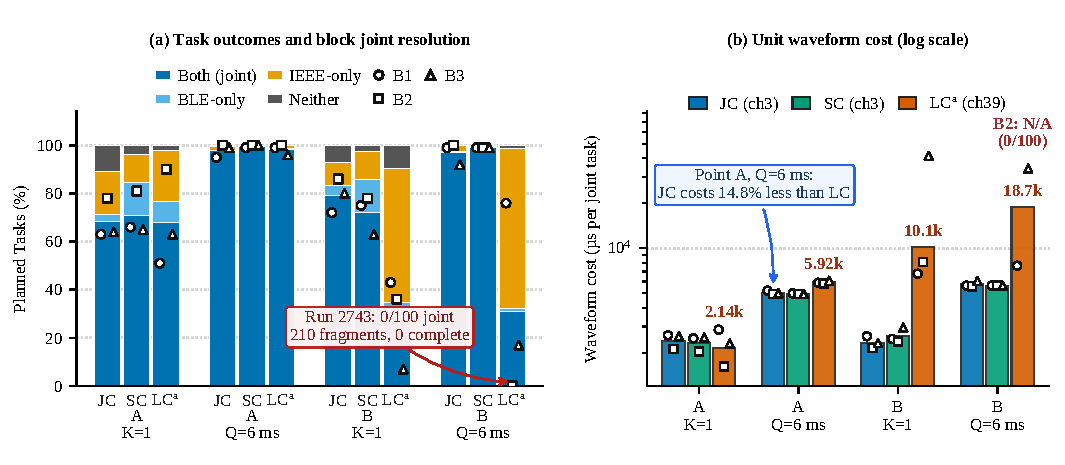
\includegraphics[width=\textwidth]{fig-p4-tradeoff.pdf}
  \caption{部分缺失无线条件 \texttt{R1} 下 36 轮确认性实验（\num{3600} 项计划任务）的四分类结果与单位波形代理成本（$K$ 为单任务计划尝试次数；$Q$ 为单任务波形预算上限，在 \SI{6000}{\micro\second} 下为 \modejc{}/\modesc{}/\modelc{}$^{\ast}$ 分别分配 A 点 $K{=}3/3/4$、B 点 $K{=}3/3/2$）：(a) 计划任务占比（\%），四分类堆叠柱分母为 $300$（合并三区组），B1/B2/B3 散点分母为 $100$（各区组独立比例；如 B 点同预算 \modelc{}$^{\ast}$ 合并联合成功柱为 $93/300$，三点依次为 $76/100$、$0/100$、$17/100$）；(b) 单位联合成功任务提交波形代理成本（对数坐标；柱为三区组总提交波形成本除以总联合成功任务数，点为各区组单轮单位成本；B2 轮次 2743 因零成功单轮记 \texttt{N/A}，其提交成本仍计入合并分子，三区组合并单位成本为 \SI{18735.5}{\micro\second}/联合成功任务；\modelc{}$^{\ast}$ 使用 \ble{} ch39，\modejc{}/\modesc{} 使用 ch3）。}
  \label{fig:p4_tradeoff}
\end{figure*}

\subsection{部分缺失无线条件 \texttt{R1} 下的成本与联合解析权衡}\label{sec:eval_p4}

P4 全部 36 轮确认性实验（\num{3600} 项计划任务）均通过采集与一致性门禁核验：全部接收摘要状态为 \texttt{complete}，队列溢出总数为 $0$，最大削波占比为 $0.00$，板端提交完成率 $100\%$ 且失败数为 $0$，全部 12 份跨模式比较记录均满足配置一致。表~\ref{tab:p4_main} 与图~\ref{fig:p4_tradeoff} 汇总了 12 个条件单元的计划尝试内联合解析率、四分类分布及单位成功任务波形代理成本。

\textbf{短负载 A 点（$b{=}0, z{=}0$，传统广播无需分片）：}如表~\ref{tab:budget} 所示，无需分片的 \modelc{} 单次尝试波形代理最低（\SI{1456}{\micro\second}，\modejc{}/\modesc{} 为 \SI{1648}{\micro\second}）。在单次尝试（$K{=}1$）条件下，三模式合并联合解析率接近（\modejc{} $68.3\%$ 即 $205/300$，\modesc{} $70.7\%$ 即 $212/300$，\modelc{} $68.0\%$ 即 $204/300$），因此 \modelc{} 取得最低的合并单位成功成本（\SI{2141.2}{\micro\second}/任务，低于 \modesc{} 的 \SI{2332.1} 与 \modejc{} 的 \SI{2411.7}{\micro\second}/任务）。然而在同预算上限 $Q{=}\SI{6000}{\micro\second}$ 下（\modejc{}/\modesc{} 分配 $K{=}3$，\modelc{} 分配 $K{=}4$），三模式计划尝试内联合解析率均逼近饱和（\modejc{} $98.0\%$、\modesc{} $99.7\%$、\modelc{} $98.3\%$）；由于开环 \modelc{} 仍为全部任务消耗了第 $4$ 次尝试（总提交 \SI{1747200}{\micro\second}，仅余 \SI{52800}{\micro\second} 未用预算），而 \modejc{}/\modesc{} 在 $K{=}3$（总提交 \SI{1483200}{\micro\second}，保留 \SI{316800}{\micro\second} 未用预算）下已接近全收，单位成功任务成本排序随策略发生翻转：\modejc{}（\SI{5044.9}{\micro\second}/任务）与 \modesc{}（\SI{4960.5}{\micro\second}/任务）分别比 \modelc{}（\SI{5922.7}{\micro\second}/任务）低约 $14.8\%$ 与 $16.2\%$（图~\ref{fig:p4_tradeoff}(b)）。

\textbf{长负载 B 点（$b{=}26, z{=}0$，结构差异与无线观测）：}从协议结构看，面对 \SI{52}{B} \ble{} 记录，\modejc{} 与 \modesc{} 仍以单个次信道数据单元完整承载（\SI{1856}{\micro\second}/尝试，$Q{=}\SI{6000}{\micro\second}$ 下分配 $K{=}3$），而 \modelc{} 须切分为 $5$ 片 \fragproto{} 分片（$6$ 突发、\SI{2904}{\micro\second}/尝试，同预算下被压缩至 $K{=}2$）。在所测 ch3 \modejc{} 对 ch39 \modelc{} 无线配置下，三个独立区组均观察到 \modejc{} 较高的联合解析率：$K{=}1$ 时 \modejc{} 均值 $79.3\%$（$238/300$）对比 \modelc{} $28.7\%$（$86/300$），逐区组差值为 $+29/+50/+73$\,pp（均值 $+50.67$\,pp，$95\%$ $t$ 区间 $[-4.00, +105.34]$\,pp），合并单位成功成本低 $76.9\%$（\SI{2339.5} vs.\ \SI{10130.2}{\micro\second}/任务）；$Q{=}\SI{6000}{\micro\second}$ 时 \modejc{} 均值 $97.0\%$（$291/300$）对比 \modelc{} $31.0\%$（$93/300$），逐区组差值为 $+23/+100/+75$\,pp（均值 $+66.00$\,pp，$95\%$ $t$ 区间 $[-31.58, +163.58]$\,pp），合并单位成功成本低 $69.4\%$（\SI{5740.2} vs.\ \SI{18735.5}{\micro\second}/任务）。必须指出两项边界：其一，受限于 $n{=}3$ 区组（$\text{df}{=}2$）小样本 $t$ 近似与区组间大幅波动，两项置信区间均跨零且端点超出 $\pm 100$\,pp，因此不宣称统计显著；其二，由于 \modejc{}/\modesc{} 使用 ch3 而 \modelc{} 使用 ch39，上述差距严格限定于所测封装与信道组合，不能单独归因于格式。分片级记录直观揭示了完成条件的苛刻性（图~\ref{fig:p4_tradeoff}(a)）：在 B2 轮次 2743（\modelc{}，$Q{=}\SI{6000}{\micro\second}$，$K{=}2$）中，\stdfour{} 侧独立恢复 $98/100$ 项任务，\ble{} 侧共收到 $210$ 个有效 \fragproto{} 分片，但无任何一次尝试集齐全部五片，最终完整重组为 $0$（\texttt{zigbee\_only} $=98/100$，联合成功 $0/100$，单轮单位成本 \texttt{N/A}）；B3 轮次 2761 与 2764 分别收到 $306$ 与 $615$ 片，但仅完整重组 $9$ 与 $19$ 条（联合成功 $7/100$ 与 $17/100$）。现有日志无法识别单个分片缺失的具体物理成因；若用 $p^5$ 刻画重组概率，还需额外假设五片接收相互独立且成功概率相同。

\textbf{同频公平对照（\modejc{} 对 \modesc{}）：}在相同频点（\ble{} ch3、\stdfour{} ch12，$12/12$ 满足协议归因检查）下，四组条件的 $\modejc{}-\modesc{}$ 均值差依次为 A-$K{=}1$ $-2.33$\,pp（$[-5.20, +0.54]$）、A-$Q$ $-1.67$\,pp（$[-6.84, +3.50]$）、B-$K{=}1$ $+7.33$\,pp（$[-17.55, +32.22]$）与 B-$Q$ $-2.00$\,pp（$[-12.83, +8.83]$），置信区间均跨零。在已测条件下，三个区组未显示 \modejc{} 相对 \modesc{} 稳定的联合解析优势（配置匹配与区间跨零均不能证明两者统计等效）。从四分类描述性分布看（图~\ref{fig:p4_tradeoff}(a)），$K{=}1$ 合并 300 项任务中，\modejc{} 呈现更少的 \texttt{ble\_only} 与更多的共同缺失 \texttt{neither}——A 点 \modejc{} 为 $9/300$ 与 $33/300$，而 \modesc{} 为 $42/300$ 与 $12/300$；B 点 \modejc{} 为 $12/300$ 与 $21/300$，而 \modesc{} 为 $41/300$ 与 $8/300$（本文不对双侧相关性作形式假设检验），这一形态与共享或分离次信道射频突发的结构一致。由此，\modejc{} 相对同频 \modesc{} 可直接确认的结构收益在于：在相等的单次尝试提交波形代理预算下将突发数由 $3$ 次减至 $2$ 次，并提供经同 IQ 核验的固定包内位置偏移以支撑共包时间参考。

% ============================================================
%  表 III（中文伴生版）：与 ../tables/tab-p2-time.tex 数值 100% 同步
%  数据源：python/experiments/p5_freeze_20261124/p5_p2_h5.csv
% ============================================================
\begin{table}[t]
\centering
\caption{固定次信道时间参考留出残差与单侧馈线断开恢复实例（轮次 2715--2717，\texttt{time} 配置）}
\label{tab:p2_time}
\setlength{\tabcolsep}{1.2pt}
\scriptsize
\begin{tabular}{@{}llccccccc@{}}
\toprule
\textbf{轮} & \textbf{场景} & \textbf{联合} & \multicolumn{2}{c}{\textbf{覆盖}} & \multicolumn{2}{c}{\textbf{计划内恢复}} & \multicolumn{2}{c}{\textbf{中位/P95 (ms)}} \\
\cmidrule(lr){4-5}\cmidrule(lr){6-7}\cmidrule(lr){8-9}
 & & 任务 & B & Z & B & Z & B & Z \\
\midrule
2715 & 正常   & 6/6 & 24/24 & 24/24 & N/A(0/0) & N/A(0/0) & .223/.318 & .129/.295 \\
2716 & B断馈  & 5/6 & 19/24 & 24/24 & 1/1      & N/A(0/0) & .242/.395 & .144/.330 \\
2717 & Z断馈  & 5/6 & 24/24 & 19/24 & N/A(0/0) & 1/1      & .222/.317 & .134/.336 \\
\bottomrule
\end{tabular}
\par\smallskip
\raggedright\scriptsize
三轮均采用 \texttt{R0} 馈线直连拓扑，每轮 $300$ 槽（周期 \SI{500}{ms}：$6$ 项任务 $\times$ $K{=}3$ 与 $282$ 个等长纯时间更新槽；双侧共覆盖探针的估计差中位数为 \SIrange{0.140}{0.153}{ms}、P95 为 \SIrange{0.202}{0.264}{ms}，$n{=}24,19,19$）。按 \texttt{uc1\_time\_tail\_audit} 口径将停发后尾段 \texttt{stale}（双侧各 $1/1$）与计划内事件分离；未受干预侧无计划内失更事件，记为 \texttt{N/A (0/0)}。每轮均有 $0/6$ 项计划任务通过定时软件处理判定（外部射频参考界未校准）。表中数据为本侧 IQ 采样域留出绝对预测误差，不代表跨设备时钟同步精度。
\end{table}


\subsection{固定次信道时间参考与单侧馈线断开恢复}\label{sec:eval_time}

表~\ref{tab:p2_time} 给出了 \texttt{R0} 馈线直连拓扑下三轮 \texttt{time} 配置（B 点 \modejc{}，每轮 $300$ 槽含 $282$ 个等长纯时间更新槽，按 \texttt{uc1\_time\_tail\_audit} 口径将停发后录制尾段 \texttt{stale} 与计划内事件分离）的观测结果。无干预基线（轮次 2715）中，双侧联合解析 $6/6$ 项任务且留出时间探针覆盖均为 $24/24$，\ble{} 与 \stdfour{} 本侧 IQ 采样域绝对预测残差中位数分别为 \SI{0.223}{ms}（P95 \SI{0.318}{ms}）与 \SI{0.129}{ms}（P95 \SI{0.295}{ms}）。在轮次 2716（人工断开 \ble{} 侧馈线）与 2717（人工断开 \stdfour{} 侧馈线）中，现场笔记记录了人工干预的大致包序范围；未受干预侧始终维持 $24/24$ 留出探针覆盖且计划内失更事件为 $0$ 次（恢复率记 \texttt{N/A (0/0)}）；在断开馈线与恢复接收的过程中，受干预侧先后出现 \texttt{holdover}、\texttt{stale}、\texttt{reacquiring} 与 \texttt{tracking}，各取得 $1/1$ 计划内恢复（留出探针覆盖 $19/24$，联合任务 $5/6$）。按受干预接收机本侧 IQ 采样索引计时，从进入 \texttt{stale} 至恢复 \texttt{tracking} 的时长在 2716（\ble{} 侧）与 2717（\stdfour{} 侧）分别为 \SI{23.0}{s}（\SI{23003.1}{ms}）与 \SI{24.0}{s}（\SI{24002.6}{ms}）；其中，重获训练（从首次进入 \texttt{reacquiring} 至恢复 \texttt{tracking}，每轮均收集 $8$ 个训练包）分别耗时约 \SI{7.0}{s}（\SI{6996.0}{ms}）与 \SI{9.0}{s}（\SI{8994.8}{ms}）。三轮实验的定时处理均因缺少外部校准参考界而保守拒绝（$0/6$）。上述数据作为共包时间参考机制的可用性与失更恢复功能实例，不与 X-Sync~\cite{hofmann2021xsync} 等跨设备绝对同步精度直接对比。

\section{讨论与结论}\label{sec:conclusion}

\emph{主要结论与设计启示：}本文明确了在单发送机约束下将双协议命令共包于单个 \ble{}~5 \texttt{AUX\_ADV\_IND} PDU 何时能在结构、成本与可靠性上获得实际收益。第一，\proto{} 在单包内稳定承载 $26/26$、$52/26$ 与 $28/32$\,B 的 \ble{}/\stdfour{} 完整记录及确定性 $400{+}8b\,\si{\micro\second}$ 包内偏移，在相等单次尝试提交波形时长下将同频每次尝试突发数由 $3$ 减至 $2$（\modejc{} 对 \modesc{}），既不损失计划尝试内联合解析率，也能支撑固定次信道本地时间可用性与单侧断馈恢复。第二，针对无需分片的短命令（$26/26$\,B），传统 \modelc{} 在 $K{=}1$ 时单位成本最低，但在 \SI{6}{ms} 重发预算上限下，\modejc{} 与 \modesc{} 在 $K{=}3$ 即已饱和而 \modelc{} 仍须发射第四次，使单位成本排序发生反转（\modejc{} 低 $14.8\%$、\modesc{} 低 $16.2\%$）；这说明在受限预算策略下，单包大小并非决定累积成本的唯一因素，重发粒度同样关键。第三，当 \ble{} 净荷超过 \SI{27}{B} 直接上限（$52/26$\,B）时，单次信道 PDU 共包免除了五分片 \fragproto{} 的全有或全无重传脆弱性，使 ch3 \modejc{} 在全部三个区组中均高于 ch39 \modelc{}（$K{=}1$ 时 $238/300$ 对 $86/300$；\SI{6}{ms} 时 $291/300$ 对 $93/300$），单位成本降低 $69.4\%\text{--}76.9\%$。

\emph{有效性边界与后续工作：}四项边界制约上述结论的外推：（i）ch3 \modejc{}（\SI{2410}{MHz}）与 ch39 \modelc{}（\SI{2480}{MHz}）对比将格式与载频耦合在一起，$n{=}3$ 区组（$\text{df}{=}2$）下小样本 $t$ 区间跨零，且 B1 点未测量无线单位成本；（ii）成本度量基于 DMA 提交基带时长而非功率计 RF 能耗或切频开销，同时未校准的接收时钟使全部 \num{2730}/\num{3600} 项已联合解析任务的截止期前交付合规不可判定（其余 \num{870}/\num{3600} 项未完成联合解码）；（iii）\stdfour{} 偏移补偿依赖预共享 $b$ 值；（iv）固定次信道 SDR 测试台尚未验证商用 \ble{}/ZigBee 协议栈互操作、动态 \texttt{AuxPtr} 在线时间维持与物理执行器同步。后续工作将引入共享时钟 RF 仪表、同信道对照、商用 \ble{}~5/\stdfour{} 芯片及动态 \texttt{AuxPtr} 跟随以审计严格截止期。


\bibliographystyle{IEEEtran}
\bibliography{refs}

\end{document}
